\documentclass[12pt]{article}

%---------------------------------
%中文设置
\usepackage[UTF8]{ctexcap}
\setCJKsansfont[ItalicFont={黑体}]{宋体}
\renewcommand\CJKfamilydefault{\CJKsfdefault}
\setCJKmonofont{仿宋}

%英文字体
\setmainfont{Times New Roman}


\renewcommand{\figurename}{图}
\renewcommand{\contentsname}{目录}
\renewcommand{\abstractname}{摘要}
\renewcommand{\refname}{参考文献}
\setlength{\parindent}{3em}
%图表标题设置
\usepackage[margin=9pt, font=small, labelfont=bf,labelsep=quad]{caption}

%中英双标题
%\bicaption{中文标题}{English title}
\usepackage{bicaption}[2012/04/09 v1.1]

\captionsetup[figure][bi-first]{name=图}
\captionsetup[figure][bi-second]{name=Figure}

\captionsetup[table][bi-first]{name=表}
\captionsetup[table][bi-second]{name=Table}

\usepackage{enumitem}
%----------------------------------
%页面设置
%使\section中的内容左对齐
\usepackage[raggedright]{titlesec}

\setcounter{secnumdepth}{4}

\titleformat{\paragraph}
{\normalfont\normalsize\bfseries}{\theparagraph}{1em}{}
\titlespacing*{\paragraph}
{0pt}{3.25ex plus 1ex minus .2ex}{1.5ex plus .2ex}

%页面边距

\usepackage{geometry}
\geometry{left=0.5in, right=0.5in}

%页眉页脚
%\usepackage{fancyhdr}
%\pagestyle{fancy}
%\fancyhead[L]{多功能职工文化中心 计算书}
%\fancyhead[R]{结32 王超杰 2013010179}

%页边距
\usepackage{geometry}
\geometry{left=2.5cm,right=2.5cm,top=2.5cm,bottom=2.5cm}

%---------------------------------
%matlab代码显示
%\usepackage[framed,numbered,autolinebreaks,useliterate]{mcode}

%---------------------------------
%数学符号显示
\usepackage{amssymb}
\usepackage{amsmath}
\usepackage{bm}

%---------------------------------
%罗马数字定义
\makeatletter
\newcommand{\rmnum}[1]{\romannumeral #1}
\newcommand{\Rmnum}[1]{\expandafter\@slowromancap\romannumeral #1@}
\makeatother

%\renewcommand{\labelenumi}{\roman{enumi}}

%---------------------------------
%方程组
%\begin{equation}
%   \left\{
%   \begin{aligned}
%       &x_2 =0\\
%       &x_1 =0\\
%       &x_1 =1\\
%       &x_2(1-x_1)^4 =1
%   \end{aligned}
%   \right.
%\end{ }

%---------------------------------
%插图
\usepackage{graphicx}

%单图
%\begin{figure}[!htbp]
%  \centering
%  \includegraphics[width=0.7\textwidth]{ }
%  \caption{ }
%  %\label{ }
%\end{ }

%单图不浮动
\usepackage{float}
%\begin{figure}[H]
%   \centering
%   \includegraphics[ ]{ }
%   \caption{ }
%\end{ }

%文字绕排
\usepackage{wrapfig}
%\begin{wrapfigure}[<行数>]{<位置>l/r}[<外伸长度>}]{<宽度>}
%   \centering
%   \caption{ }
%   \includegraphics[ ]{ }
%\end{ }

%双图
%\begin{figure}
%   \centering
%   \caption{ }
%   \includegraphics[ ]{ }
%       \subcaption{ }
%   \qquad
%   \includegraphics[ ]{ }
%       \subcaption{ }
%\end{ }

%---------------------------------
%标题
\usepackage{caption, subcaption}
%\captionsetup{font = {small, sf}, labelfont = bf}
%字号选择:
%- scriptsize
%- footnotesize
%- small
%- normalsize
%- large
%- Large
%
%字体族:
%- rm 罗马体
%- sf 无衬线体
%- tt 打字机体
%
%字体系列:
%- md 中等粗细
%- bf 粗体
%
%字体形状:
%- up 直立体
%- it 意大利体
%- sl 倾斜体
%- sc 小型大写字母

%---------------------------------
%表格
\usepackage{longtable}
\usepackage{booktabs}
\usepackage{bigstrut}
\usepackage{multirow}

\usepackage{chngpage}
%\begin {table}[H]
%\caption{This is a long table}
%\begin{adjustwidth}{-3cm}{} %第一个参数为调整左页边距,第二个参数右页边距可置空
%\end{adjustwidth}
%\end{table}

\usepackage{import}
%---------------------------------
\def\tightlist{}

%---------------------------------
\begin{document}

\title{ 磁流变液\\
	MRF}
\date{}
\author{王超杰\and 吕晚晴\and 苗增辉\and 林超超}

\maketitle

%---------------------------------
\abstract

\thispagestyle{empty}
\newpage
\tableofcontents
\thispagestyle{empty}
\newpage
\setcounter{page}{1}

%---------------------------------

\section{引言}
\subsection{绪论}
\subsection{结构振动控制问题研究现状}
1972年,Yao最初提出土木工程结构振动控制的概念\cite{yao1972concept}。其基本思想是在结构中安装特定的控制装置,对结构施加控制力或调整动力性能。经过近半个世纪的发展,从外界能量输入的角度可以将结构振动控制分为被动控制、主动控制和半主动控制三种。

\subsubsection{被动控制}
被动控制利用隔震、减震装置隔离、吸收振动,保护主体结构,防止振动在结构中传播。被动控制系统构造简单、不依赖于外界供能,主要可分为基础隔震、耗能减震和调谐减震三种方式。
\begin{enumerate}
	\item 基础隔震最早由日本学者河合浩藏于1881年提出,指在建筑物或构筑物基底设置夹层,阻止地震能量向基础以上传播。基础隔震不仅适用于一般的多层建筑,也已成功应用于桥梁的振动控制。但是,基础隔震控制效果有限,无法适应高层建筑的抗震需求\cite{Sun2012}。
	\item 耗能隔震系统将阻尼等耗能吸震装置设置在结构的节点等连接处,在外界激励下,耗能装置首先进入弹性甚至非弹性状态,发生较大变形,大量吸收外力能量,保护主体结构。耗能装置便于维护、更换,性能发挥稳定,但对一栋大型建筑而言,耗能装置体量显著提升,成本较高。
	\item 调谐减震系统增设局部的子结构,通过子结构与主体结构之间的刚度、自振周期及质量之间的关系减小主体结构振幅,将振动能量转移给子结构。这也是目前广泛采用的动力吸振器的原理。假设一双自由度体系,在动力荷载作用下的振动方程为:
	\begin{equation}
	\label{vibration}
	\left\{
	\begin{array}{rl}
	m_1\ddot{y_1}\left(t\right)+k_{11}y_1\left(t\right)+k_{12}y_2\left(t\right)&=F_{P1}\left(t\right)\\
	m_2\ddot{y_2}\left(t\right)+k_{21}y_1\left(t\right)+k_{22}y_2\left(t\right)&=F_{P2}\left(t\right)
	\end{array}
	\right.
	\end{equation}
	假设外界激励为简谐荷载,即:
	\begin{equation}
	\label{sin}
	\left\{
	\begin{array}{rl}
	F_{P1}\left(t\right)&=F_{P1}\sin \theta t\\
	F_{P2}\left(t\right)&=F_{P2}\sin \theta t
	\end{array}
	\right.
	\end{equation}
	在平稳振动阶段,各质点也将做简谐振动,即:
	\begin{equation}
	\label{sinMove}
	\left\{
	\begin{array}{rl}
	y_{1}\left(t\right)=Y_{1}\sin \theta t\\
	y_{2}\left(t\right)=Y_{2}\sin \theta t
	\end{array}
	\right.
	\end{equation}
	
	最终可解得:
	\begin{equation}
	\label{answer}
	\left\{
	\begin{array}{rl}
	D_0&=\left(k_{11}-\theta^2m_1\right)\left(k_{22}-\theta^2m_2\right)-k_{12}k_{21} \\
	D_1&=\left(k_{22}-\theta^2m_2\right)F_{P1}-k_{12}F_{P2} \\
	D_2&=-k_{21}F_{P1}+\left(k_{11}-\theta^2m_1\right)F_{P2}
	\end{array}
	\right.
	\end{equation}
	
	当$F_2=0$,$k_2=\theta^2m_2$时,由式\eqref{answer}可知$D_0=k_2^2$,且$Y_1=0$,$Y_2=-\frac{F_p}{k_2}$,即增加子结构$m_2$后,主结构$m_1$的振动被消除。
	
	从上述求解过程也可以看出,调谐减震系统由于事先需要确定减震所需的子结构刚度、质量等条件,可调节范围窄。当外界激励离设计值偏差较大时,抗震效果不能令人满意。
	
	下图就展示了一个由单自由度振子和其下方的动力吸振器组成的振动系统。对于这样一个系统,激振频率与主体结构的振幅的关系由下图中的曲线描述,可以看到,只有在外界激振力的频率处于一个很小的范围(图上阴影区域)时,动力吸振器才能够发挥减小主体结构振动的作用。事实上,上述主体结构-吸振器的系统相当于一个双自由度系统,该系统的两个主振频率分布在原来的主体结构的自振频率的两侧,从而导致动力吸振器的作用频率范围窄,对于主体结构的控制效果并不理想\cite{chopra2007}。
	
	\begin{figure}[H]
		\centering
		\bicaption{(a):单自由度系统动力吸振器;(b):响应幅度-激振频率曲线}
		{(a):Vibration absorber attached to an SDF system; (b): Reponse amplitude versus exciting frequency (dashed curve indicates negative $u_{1o}$ or phase opposite to excitation); $\mu=0.2$ and $\omega_1^*=\omega_2^*$.}
		\label{double}
		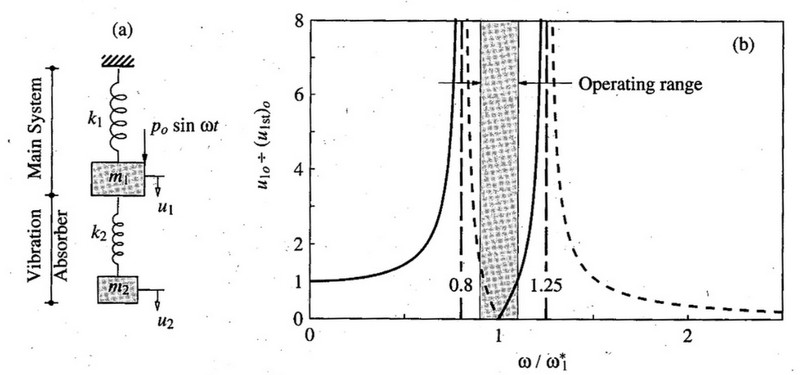
\includegraphics[width=4in]{figure/double}
	\end{figure}
	
\end{enumerate}


\subsubsection{主动控制}
结构主动控制利用外界功能,在结构受风荷载、地震荷载等情况下受激励振动的过程中,通过施加控制力或改变结构的自振周期、阻尼比等动力性能,迅速改变结构在外激励下的响应,从而控制结构振动。

主动控制系统可以分为主动质量阻尼系统(Active Mass Drive, AMD)、主动拉索系统ATS(Active Tendon System, ATS)、主动斜撑系统(Active Brace System, ABS)等。主动控制系统的工作模式可概述如下:传感器检测结构的动力响应和外部激励,将检测的信息传入计算机内,计算机根据给定的算法计算出控制力的大小,最后由AMD控制系统是主动控制系统的代表。1989年,日本东京建成世界上第一座采用AMD系统的大楼——Kyobasi Seiwa大厦\cite{T.KoboriN.KoshikaN.Yamada1991}。

随着控制算法的进步与计算机处理大规模实时数据能力的提升,主动控制系统的理论体系日趋完善,且控制效果十分出色,然而其大规模应用仍受到一些现实条件的制约:
\begin{enumerate}
	\item 严重依赖外界供能。主动控制系统完全依赖外界巨大的电能供应控制结构响应,在地震、风灾等极端条件下,电网安全难以保证,主动控制系统可能完全失效,而这恰恰是最需要结构控制的时候;
	\item 作动器吨位大,占据宝贵的建筑空间\cite{lou2013};
	\item 造价和运行维护成本高昂。
\end{enumerate}

\subsubsection{半主动控制}
结构振动的半主动控制是一种振动系统的参数控制技术,它根据系统输入的变化和对系统输出的要求,实时调节系统中元件的刚度、惯性或阻尼特性,从而改变结构的动力性能,达到控制结构振动的目的。

与被动控制系统相比,半主动控制系统的调节精度和控制范围远高于前者,对于控制建筑结构中随机性较大的地震动、风震有着良好的适应性。

半主动控制系统利用与结构的相对运动,只能向结构施加与其运动方向相反的控制力,无法实现完全主动的控制力,并且在控制精度和效果上不如主动控制系统;但是,半主动控制系统的作动器相较于主动控制系统而言成本较低,体积与重量也更易于被接受;此外,自供能的半主动控制系统利用结构往复振动产生的动能,对外界的能量输入依赖较低,克服了主动控制系统的能源问题。

综合以上论述,可以看到,半主动控制系统兼具了控制效果良好、设备简单经济的特点。

常见的半主动控制系统有:
\begin{enumerate}[leftmargin=*,labelindent=16pt,label=\bfseries \arabic*.]
	\item 主动调谐质量阻尼系统(Tuned Mass Damper, TMD),如台北101大厦的抗震体系;
	\item 可变刚度系统(Active Variable Stiffness, AVS),通过控制某些锁定装置,快速改变结构刚度,避开与外激励的共振频率,从而降低结构振幅响应。\cite{Lijing2006}显然,对于一般建筑,刚度设计值较大,为了能够提高控制效果,AVS的刚度要求较大,设计和经济意义上缺乏可行性。因此,AVS一般只应用于控制柔性结构;
	\item 可变阻尼系统(Active Viscosity System, AVS)通过调节元件中的阻尼大小,针对特定的外界激励提供相应的阻尼力,使其达到该激励下的理论最优控制力,工作模式接近主动控制系统,控制精度较高,且调节范围宽广且连续。然而,AVS控制系统中,阻尼大小一般只由速度控制,换言之,AVS无法控制结构位移;
\end{enumerate}

振动的半主动控制所涉及的关键技术是设计并实现可控减振环节与控制策略。\cite{Hu2001}可控减振环节可以具体分为可控弹性和惯性元件、可控阻尼器以及可控动力吸振器等几种类型。控制策略则以基于结构动力模型的控制策略为主,近年来,也出现了机器学习、人工神经元网络为代表的智能控制策略。

在后文中将提到的实验模型中,我们选择以可控阻尼器作为可控减震环节,控制策略则是基于模型的动力特性的算法。

\subsection{磁流变液与磁流变阻尼器}
\subsubsection{磁流变液(Magneto-Rheological Fluids(MRFs))}
磁流变液是研发于上世纪50年代的一种智能材料。典型的磁流变液由软磁性颗粒、粘滞流体和添加剂3种组分组成。在添加剂的作用下,软磁性颗粒与粘滞流体形成稳定均一的液态混合物,能够对外加磁场作出响应。

在没有外加磁场作用时,磁流变液的流变特性接近牛顿流体;在施加了外加磁场后,磁流变液则由牛顿流体转变为宾汉姆流体,即具有了一定的剪切屈服应力,并且,磁流变液的剪切屈服应力随着外加磁场的增强而连续增大,剪切屈服强度与外加磁场的磁感应强度大致呈正比例关系。

磁流变液在较大的磁感应强度变化范围内均呈现出上述的线性连续的“磁变特性”;同时,磁流变液对于外加磁场的响应时间达到毫米级,响应十分灵敏迅速\cite{Ali2015}。
此外,在一定的磁感应强度下,磁流变液达到剪切屈服应力后,磁流变液的滞回曲线十分饱满,具有良好的耗能性能,是一种理想的阻尼材料。

\subsubsection{磁流变阻尼器(MR Damper)}
磁流变阻尼器是以磁流变液作为阻尼材料的粘滞阻尼装置。

根据磁流变液在磁场作用下流变特性可控的特点,磁流变阻尼器可以根据结构的振动响应实时调整阻尼力,实现对结构振动的实时控制。可以看到,磁流变阻尼器具有阻尼力可调倍数高、响应时间短的特点\cite{Zhang2010}。

上面提到,主动控制系统中的作动器需要较大的能量输入,这一方面增加了控制系统的维护成本;另一方面也降低了系统在地震等环境下正常工作的可靠度。与之相比,磁流变阻尼器的驱动电压较低($10V$以内),借助结构的往复运动的能量,易于实现控制系统的自供能运转,提高了整个系统的可靠度。

与传统的阻尼材料相比,单位体积(或单位质量)的磁流变液能够提供更大的阻尼力,因此磁流变阻尼器具有较小质量与体积,节约了建筑空间,减轻了结构自重。



\section{结构振动控制问题研究现状}
1972年,Yao最初提出土木工程结构振动控制的概念\cite{yao1972concept}。其基本思想是在结构中安装特定的控制装置,对结构施加控制力或调整动力性能。经过近半个世纪的发展,从外界能量输入的角度可以将结构振动控制分为被动控制、主动控制和半主动控制三种。

\subsection{被动控制}
被动控制利用隔震、减震装置隔离、吸收振动,保护主体结构,防止振动在结构中传播。被动控制系统构造简单、不依赖于外界供能,主要可分为基础隔震、耗能减震和调谐减震三种方式。\cite{Zhou1997}
\begin{enumerate}
\item 基础隔震最早由日本学者河合浩藏于1881年提出,指在建筑物或构筑物基底设置夹层,阻止地震能量向基础以上传播。基础隔震不仅适用于一般的多层建筑,也已成功应用于桥梁的振动控制。但是,基础隔震控制效果有限,无法适应高层建筑的抗震需求。\cite{Sun2012}
\item 耗能隔震系统将阻尼等耗能吸震装置设置在结构的节点等连接处,在外界激励下,耗能装置首先进入弹性甚至非弹性状态,发生较大变形,大量吸收外力能量,保护主体结构。耗能装置便于维护、更换,性能发挥稳定,但对一栋大型建筑而言,耗能装置体量显著提升,成本较高。
\item 调谐减震系统增设局部的子结构,通过子结构与主体结构之间的刚度、自振周期及质量之间的关系减小主体结构振幅,将振动能量转移给子结构。这也是目前广泛采用的动力吸振器的原理。假设一双自由度体系,在动力荷载作用下的振动方程为:
\begin{equation}
\label{vibration}
\left\{
\begin{array}{rl}
m_1\ddot{y_1}\left(t\right)+k_{11}y_1\left(t\right)+k_{12}y_2\left(t\right)&=F_{P1}\left(t\right)\\
m_2\ddot{y_2}\left(t\right)+k_{21}y_1\left(t\right)+k_{22}y_2\left(t\right)&=F_{P2}\left(t\right)
\end{array}
\right.
\end{equation}
假设外界激励为简谐荷载,即:
\begin{equation}
\label{sin}
\left\{
\begin{array}{rl}
F_{P1}\left(t\right)&=F_{P1}\sin \theta t\\
F_{P2}\left(t\right)&=F_{P2}\sin \theta t
\end{array}
\right.
\end{equation}
在平稳振动阶段,各质点也将做简谐振动,即:
\begin{equation}
\label{sinMove}
\left\{
\begin{array}{rl}
y_{1}\left(t\right)=Y_{1}\sin \theta t\\
y_{2}\left(t\right)=Y_{2}\sin \theta t
\end{array}
\right.
\end{equation}

最终可解得:
\begin{equation}
\label{answer}
\left\{
\begin{array}{rl}
D_0&=\left(k_{11}-\theta^2m_1\right)\left(k_{22}-\theta^2m_2\right)-k_{12}k_{21} \\
D_1&=\left(k_{22}-\theta^2m_2\right)F_{P1}-k_{12}F_{P2} \\
D_2&=-k_{21}F_{P1}+\left(k_{11}-\theta^2m_1\right)F_{P2}
\end{array}
\right.
\end{equation}

当$F_2=0$,$k_2=\theta^2m_2$时,由式\eqref{answer}可知$D_0=k_2^2$,且$Y_1=0$,$Y_2=-\frac{F_p}{k_2}$,即增加子结构$m_2$后,主结构$m_1$的振动被消除。

从上述求解过程也可以看出,调谐减震系统由于事先需要确定减震所需的子结构刚度、质量等条件,可调节范围窄。当外界激励离设计值偏差较大时,抗震效果不能令人满意。
\end{enumerate}


\subsection{主动控制}
结构主动控制利用外界功能,在结构受风荷载、地震荷载等情况下受激励振动的过程中,通过施加控制力或改变结构的自振周期、阻尼比等动力性能,迅速改变结构在外激励下的响应,从而控制结构振动。

主动控制系统可以分为主动质量阻尼系统(Active Mass Drive, AMD)、主动拉索系统ATS(Active Tendon System, ATS)、主动斜撑系统(Active Brace System, ABS)等。主动控制系统的工作模式可概述如下:传感器检测结构的动力响应和外部激励,将检测的信息传入计算机内,计算机根据给定的算法计算出控制力的大小,最后由AMD控制系统是主动控制系统的代表。1989年,日本东京建成世界上第一座采用AMD系统的大楼——Kyobasi Seiwa大厦\cite{T.KoboriN.KoshikaN.Yamada1991}。

随着控制算法的进步与计算机处理大规模实时数据能力的提升,主动控制系统的理论体系日趋完善,且控制效果十分出色,然而其大规模应用仍受到一些现实条件的制约:
\begin{enumerate}
\item 严重依赖外界供能。主动控制系统完全依赖外界巨大的电能供应控制结构响应,在地震、风灾等极端条件下,电网安全难以保证,主动控制系统可能完全失效,而这恰恰是最需要结构控制的时候;
\item 作动器吨位大,占据宝贵的建筑空间\cite{lou2013};
\item 造价和运行维护成本高昂。
\end{enumerate}

\subsection{半主动控制}
半主动控制属于参数控制,控制过程依赖于结构反应和外界激励信息,不直接向结构施加作用力,而是通过改变元件刚度、调节阻尼等方式改变结构的动力性能,达到控制结构振动的目的。半主动控制只能施加与结构运动方向相反的控制力,因此不能实现完全主动控制力,且在控制精度和效果上不如主动控制。但是,半主动控制系统利用结构往复振动时产生的动能,对外界的能量输入依赖较低,克服了主动控制系统的能源问题。同时,半主动控制系统的调节精度和范围远高于被动控制系统。因此兼具了控制效果良好、设备简单易行的特点。常见的半主动控制系统有:
\begin{enumerate}
\item 主动调谐质量阻尼系统(Tuned Mass Damper, TMD),如台北101大厦的抗震体系;
\item 可变刚度系统(Active Variable Stiffness, AVS),通过控制某些锁定装置,快速改变结构刚度,避开与外激励的共振频率,从而降低结构振幅响应。\cite{Lijing2006}显然,对于一般建筑,刚度设计值较大,为了能够提高控制效果,AVS的刚度要求较大,设计和经济意义上缺乏可行性。因此,AVS一般只应用于控制柔性结构;
\item 可变阻尼系统(Active Viscosity System, AVS)通过调节元件中的阻尼大小,针对特定的外界激励提供相应的阻尼力,使其达到该激励下的理论最优控制力,工作模式接近主动控制系统,控制精度较高,且调节范围宽广且连续。然而,AVS控制系统中,阻尼大小一般只由速度控制,换言之,AVS无法控制结构位移;
\end{enumerate}
\section{基于能量收割的半主动控制磁流变阻尼器}
\subsection{理论模型}
如前所述,结构振动控制作为结构抗震、抗风的核心技术,具有极强的工程需求与研究价值。半主动控制作为结构振动控制中的一类方式,兼具能耗小与智能切换控制状态的优点,是目前最具有工程应用前景的一种结构控制方法。磁流变阻尼器作为一种相对新型的智能阻尼器,具有构造简单,控制能耗低、响应速度快、出力大及可连续调节阻尼等优点,目前也正越来越多地应用于工程领域。结合半主动控制与磁流变(MR)阻尼器无疑为优化结构振动控制提供了一个高效可行的方向。然而,值得注意的是,尽管半主动控制具有能耗小的优点,但其也需要能量输入,同时磁流变阻尼器则是一种典型的直接耗能减振装置,同样也需要一定的能量输入,当其应用于桥梁等户外结构或在地震条件下工作时,不方便或可靠性不能保证的供电,大大制约了半主动控制磁流变阻尼器的应用。事实上,结构减振的过程,就是将结构振动能量耗散的过程,假如将振动的能量收集起来应用于半主动控制磁流变阻尼器的能源供给,上述制约也将迎刃而解。

因此,我们小组设计了一个基于能量收割的半主动控制磁流变阻尼器系统,利用能量收割的原理将振动能量转化为电能供给半主动控制系统与磁流变阻尼器,充分发挥半主动控制与磁流变阻尼器的优势,以达到更优的结构减振效果。系统理论模型如图XXX所示。

\begin{figure}[H]
\caption{系统理论模型概念图}
\end{figure}

系统工作原理如下:XXXX

由此可见,该系统主要分为MR阻尼器、能量收割模块与半主动控制模块三个部分。由于MR阻尼器的现有研究与工程应用已经相对成熟,我们并未在MR阻尼器的构造上进行过多地创新,仅根据结构特点与需求设计了“双出型”磁流变阻尼器,对其力学性质进行数值模拟与试验测试。针对能量收割模块,我们分析讨论在结构振动控制领域能量收割的一些方式,为验证能量收割的可行性,测算能量转换效率,制作了一个直线型电磁感应能量收割装置进行试验。对于半主动控制模块,XXXX

\subsection{振动能量收割原理及实现方式}

所谓能量收割(Energy Harvesting),是指通过特定方式将通常直接消耗或废弃的能量转化为其他更有用的能量形式。而土木工程结构由于风荷载、地震激励或人致激励产生的振动能就是一种通常直接消耗或废弃的能量,由于结构的振动无所不在,从理论上而言,这种能量非常大,这也意味着土木工程结构能够收割的能量非常大。然而,相对于航天航空、机械、电子等领域的振动能量,土木工程结构的振动能量属于低频能量,往往只有几赫兹,这使得广泛应用于高频能量收割的压电材料并不能够很好地适用于土木工程领域。

目前在土木工程领域已有的能量收割研究主要有两个方向:将振动能量转化为将振动能量转化为液压能与将振动能量转化为电能。由于半主动控制磁流变阻尼器要求的能量输入形式为电能,我们选择的能量收割途径为将振动的机械能转化为电能。静电、压电方式与电磁感应是将振动机械能转化为电能的三种形式,然而由于静电式转换机械能时需要外部电源提供静电场,与我们的目的相悖,而压电式能量转换系统并不能够很好地适用于低频的振动机械能转换。因此,我们选用电磁感应能量转换系统来实现能量收割。

电磁感应能量转换系统,通俗而言,就是应用电磁感应技术进行发电的发电机。电磁感应技术是一项非常成熟,应用发展也非常完善的发电技术。相比于压电能量捕获技术,电磁感应技术电能转换效率更高、发电量更大、理论技术也更为完善,最重要的是,它能够适应土木工程结构低频振动的特点,相对高效地进行结构振动能量收割。目前商用的发电机多为旋转式发电机,但考虑到结构振动是线性运动,如使用旋转式发电机,还需要增加转换装置,制作复杂,也使得机械能耗散加大,降低能量转换效率,所以我们决定根据结构特点,设计直线型发电机用于能量收割。

\subsection{最优控制力求解}
线性结构在外部激励和作动器出力的共同作用下,运动方程为
\begin{equation}
\mathbf{M \"{X} + C\.{X} +KX=F(t)+Du} \label{zongfangcheng}
\end{equation}
式中,$\mathbf{K,M,K}$为结构的质量矩阵、阻尼矩阵和刚度矩阵,$\mathbf{F(t)}$为外部激励,$\mathbf{D}$为作动器的位置向量,$\mathbf{u}$为作动器的控制力。

将式\eqref{zongfangcheng}转化为状态方程,令$\mathbf{U=\left(X,\.{X}\right)^T}$,则
\begin{equation}
\dot{\mathbf{U}}=\mathbf{AU+Bu+HF(t)}   \label{zhuangtai}
\end{equation}
式中,

\begin{equation}
\mathbf{
A=\left[
\begin{array}{cc}
0 & I \\
-M^{-1}K & -M^{-1}C
\end{array}
\right],
B=\left[
\begin{array}{c}
0 \\
M^{-1}D
\end{array}
\right],
B=\left[
\begin{array}{c}
0 \\
M^{-1}
\end{array}
\right]
}
\end{equation}

式\ref{zhuangtai}中,出力结构的状态\textbf{U}未知外,作动器的控制力\textbf{u}同样未知,所以关键是如何得到\textbf{u}.

\subsubsection{经典最优控制}
定义性能指标:
\begin{equation}
\mathbf{min\quad J=\int^{t_f}_0\left[U^T(t)QU(t)+u^T(t)Ru(t)\right]\mathrm{d}t}
\end{equation}
式中,\textbf{Q,R}为权矩阵,分别表示控制效果的权值和控制力的权值。
\begin{equation}
\mathbf{s.t.\quad} \dot{\mathbf{U}}=\mathbf{AU+Bu+HF(t)},\quad \mathbf{U(0)=U_0}  \label{dairu1}
\end{equation}

用优化的方法,可以得到
\begin{equation}
\dot{\mathbf{\lambda}}=\mathbf{-A^T\lambda-2QU,\quad \lambda(t_f)=0}
\end{equation}

\begin{equation}
\mathbf{u=-\frac{1}{2}R^{-1}B^T\lambda}
\end{equation}

方程的解已经在控制工程中得到解决,直接引用结论,作动器控制力为:
\begin{equation}
\mathbf{u=-\frac{1}{2}R^{-1}B^TPU(t)=-GU(t)} \label{konghzhili}
\end{equation}
式中,\textbf{G}称为反馈增益矩阵
\begin{equation}
\mathbf{G=\frac{1}{2}R^{-1}B^TP} \label{fankui}
\end{equation}

将欲求的控制力\textbf{u}再代入式\ref{dairu1},得
\begin{equation}
\dot{\mathbf{U}}=\mathbf{(A-BG)U+HF(t)}  \label{xianxingjiegou}
\end{equation}

式\ref{xianxingjiegou}表示一个线性结构,容易求得结构状态\textbf{U(t)}.需要注意的是,在方程求解过程中,忽略了外部激励\textbf{HF(t)},因此只是近似最优。

所以,经典最优控制算法求最优控制力步骤是
\begin{enumerate}
\item 写出结构运动方程,并转化为状态方程\ref{zhuangtai};
\item 根据式\ref{fankui},得到反馈增益矩阵\textbf{G};
\item 将\textbf{G}代入式\ref{xianxingjiegou}求解结构反应;
\item 将结构状态\textbf{U(t)}代入式\ref{konghzhili},得到作动器的最优控制力。
\end{enumerate}
\subsubsection{瞬时最优控制}
经典最优控制忽略了外部激励 \textbf{HF(t)},所以求得的最优控制力只是近似最优,同时,由于经典的最优控胡子算法的目标函数是一个积分,说明整个时间段内结构参数不变,也就是说,经典最优控制算法只能对线性结构进行求解,为了改进这些问题,Yang 提出了瞬时最优控制算法,该算法作了三点改进:
\begin{enumerate}
\item 性能指标由全部时间内的二次型最小改为每时刻的二次型最小;
\item 不再用 Ricaati 方程求解控制力,而是将状态方程变换为差分方程,差分方程中的变量只与前一时刻的值有关,这样就可以迭代求解控制力和结构的响应;
\item 瞬时最优控制的目标函数是每时刻最优,也就是说,结构仅在微小时段内为线性,所以该算法可以解决非线性结构的控制问题。
\end{enumerate}

首先定义性能指标
\begin{equation}
J=U^T(t)QU(t)+u^T(t)Ru(t)
\end{equation}
状态方程变为
\begin{equation}
U(t)=\Phi d(t-\Delta t)+\frac{\Delta t}{2}\left[Bu(t-)+HF(t)\right]  \label{dairu2}
\end{equation}


\begin{equation}
d(t-\Delta t)=e^{\lambda \Delta t}\Phi^{-1}\left\lbrace U(t-\Delta t)+ \frac{\Delta t}{2}\left[Bu(t-\Delta t)+HF(t-\Delta t)\right]\right\rbrace  \label{dairu3}
\end{equation}

然后用与经典最优控制算法相同的优化方法,求解得到
\begin{equation}
u=-\frac{\Delta t}{2}R^{-1}B^TQU(t)    \label{kongzhili2}
\end{equation}
再将式\ref{kongzhili2} 代入式\ref{dairu2},得
\begin{equation}
U(t)=\left[I+\frac{\Delta t^2}{2}BR^{-1}B^TQ\right]^{-1}\left[\Phi d(t-\Delta t) +\frac{\Delta t}{2}HF(t)\right]  \label{diedai}
\end{equation}

式\ref{diedai}是一个迭代式,由此可以求得每个时刻的响应。

因此,瞬时最优控制的步骤为:
\begin{enumerate}
\item 写出结构的运动方程,并转化为瞬时的状态方程,如式\ref{dairu2};
\item 给定结构的初始状态,用式\ref{dairu3}得到$d(t-\Delta t)$;
\item 按照式\ref{diedai}得到下一时刻结构的响应$U(t)$;
\item 按照式\ref{kongzhili2}得到下一时刻的控制力$U(t)$;
\end{enumerate}

\subsubsection{LQG控制}
XXXX

\subsection{半主动控制算法及系统}
控制算法选择的好坏直接影响控制系统的性能。对磁流变阻尼结构来货,由于磁流变阻尼器是通过调整磁场的强度来调整产生的阻尼里,接着通过调节事假在磁流变阻尼器的电压(电流)大小使其产生的阻尼里趋向于最优的控制力。有效改变电压(电流)的大小,是利用磁流变阻尼器实现有效控制的关键所在。国内外学者根据磁流变阻尼器的特显,提出了很多种控制策略。

\subsubsection{恒定加压式}
这种控制算法主要包括了 Passive-off, Passive-on 两种形式,分别指对磁流变阻尼器不施加电压和施加最大电压。

在这种恒定加压式控制算法下,磁流变阻尼器相当于一个被动阻尼器,其形式简单,操作便捷,但存在着很大的缺憾:
\begin{enumerate}
\item Passive-off 策略提供的阻尼力较小,不能使磁流变阻尼器发挥出真正的性能。
\item Passive-on 策略提供的阻尼力较大,阻尼器的内力很少有机会超过磁流变阻尼器的屈服力,因此磁流变阻尼器仅起到一个增大结构刚度的作用,未祈祷耗能减振的作用,在地震时因为刚度的增大反而可能加大地震响应。
\end{enumerate}

\subsubsection{离散加压式}
离散加压式指施加在磁流变阻尼器上的电压(电流)的大小分为几个档位,形成双态控制或者三态控制。

常见的双态控制策略一般是当磁流变阻尼器产生的阻尼力小于最优控制力,并且两者方向一致时,将输入电压调到最大,否则为零。

用双态控制对磁流变阻尼器进行控制,计算简单,控制方便,易于操作,但振动较小时容易引起阻尼力超调,使受控结构的动力反应产生局部放大的现象,引起负面效应。

为此有人提出了三态控制,控制档位增设中间一档,但虽然优于双态控制,但仍然未发挥磁流变阻尼器全部性能,控制策略仍然不够细腻。

\subsubsection{PID控制}

PID控制是比例(P)、偏差积分(I)、偏差微分(D)控制的简称。常规PID控制系统原理孔图如图所示 XXXX


\paragraph{PID控制基本原理}
控制规律为
\[\mathrm{u}(t)=\mathrm{MV}(t)=K_p{e(t)} + K_{i}\int_{0}^{t}{e(\tau)}\,{d\tau} + K_{d}\frac{de(t)}{dt}\]

其中:
$K_p$:比例增益,是调适参数\\
$K_i$:积分增益,也是调适参数\\
$K_d$:微分增益,也是调适参数\\
$e$:误差=设定值(SP)- 回授值(PV)\\
$t$:目前时间\\
$\tau$:积分变数,数值从0到目前时间t

\paragraph{PID控制器设计及参数整定}
采用PID控制策略时,$K_{k},K_{i},K_{p}$三个参数对系统的控制效果起决定性作用,采用凑试发确定 PID参数,分为以下几步:
\begin{enumerate}
\item 首先选择 $K_p$ 值得到期望的暂态响应,而置 $K_i,K_d$为零,然后逐步改变 $K_p$,同时观察系统变化,知道控制系统得到响应较好,超调小的响应曲线。此时系统仍有较大的稳态误差。
\item 加入积分环境,整定积分参数。首先置$K_i$为一个较小的值,同时变化$K_p$为较小值,不断变化$K_i$,使系统在保持良好动态性能的情况喜爱,静差得到消除。
\item 加入微分环节,构成PID控制器,微分系数$K_d$的整定方法同第二步,逐步增大$K_d$的同时相应地变化$K_p,K_i$,逐步试凑,以获得满意的调节效果和控制参数。
\end{enumerate}

\paragraph{PID控制仿真结果}
XXXX

\subsubsection{模糊控制}
磁流变阻尼器双态控制和三态控制电流的选择档次只有两档和三档,控制较为粗糙,想要实现精确地控制加入磁流变阻尼器的结构,最好实行全态控制。

为了在短暂的时间内实现全态的励磁电流选择,将模糊逻辑控制技术应用到加入磁流变阻尼器结构的全态控制中,即采用模糊逻辑控制器根据传感器所采集的机构状态信号和外界激励信号瞬时作出电流选择,所确定的电流输入到阻尼器实现对结构的全态控制。

如图 XXXX,每一时刻地震加速度和建筑结构的状态被信号检测器检测并被输入到模糊逻辑控制器中,在预定的模糊规则和隶属函数下经模糊逻辑控制器的模糊推理后,得到一控制电流,将控制电流指令信号传递给磁流变阻尼器,磁流变阻尼器产生控制力并施加给结构。这便是加有磁流变阻尼器结构的模糊逻辑全态控制的整个构思框架。

\paragraph{输入量、输出量的选取}
\qquad 模糊控制器应用比较多的是以误差和误差的变化为输入变量的二维模糊控制,选用位移与系统位移响应之间的误差$e$ 与变化率$\Delta e$作为控制器的输入量,控制电流变化的量为输出。
\paragraph{输入、输出变量的正规化处理及基本论域确定}
\qquad 在模糊控制器设计中,信号的实际变化范围称为变量的基本论域,误差变化及输出变量的变化区间,经变换得到正规化输入输出变量为:
\[x=\frac{e}{e_{max}}\qquad \qquad y=\frac{\Delta e}{\Delta e_{max}}\qquad \qquad z=\frac{I}{I_{max}}\]

其中,$x\in [-1,1]; y\in [-1,1]; z\in [0,1]$.

\paragraph{模糊集合与隶属函数的确定}
\qquad 对论域 $x,y$,定义五个模糊子集表示输入的模糊状态
\[\mathbf{\lbrace NB,NS,Z,PS,PB\rbrace}\]
输出变量$z$的模糊集合也定义五个子集表示
\[\mathbf{\lbrace Z,S,M,SB,B\rbrace}\]
模糊语言变量隶属度函数输入、输出采用高斯型如图
\begin{figure}[H]
\centering
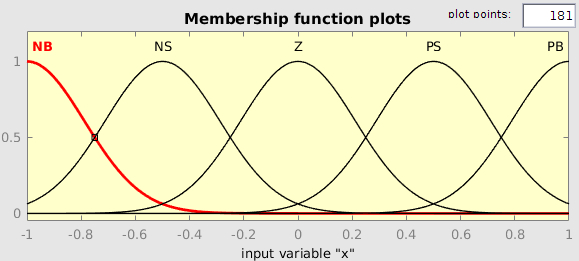
\includegraphics[width=0.5\linewidth]{figure/fuzzyx}
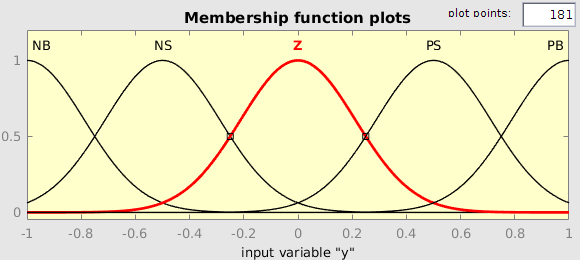
\includegraphics[width=0.5\linewidth]{figure/fuzzyy}
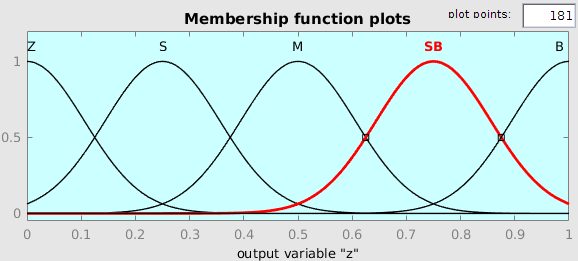
\includegraphics[width=0.5\linewidth]{figure/fuzzyz}
\end{figure}

\paragraph{模糊控制规则的确定}
\qquad 模糊控制规则采用相关参考文献的控制规律 XXXX,根据模糊推理规则,输出与位移变化及其变化率的曲面关系如图XXXX
\begin{figure}[H]
\centering
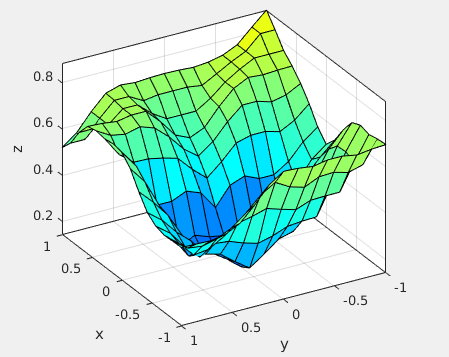
\includegraphics[width=0.5\linewidth]{figure/fuzzysurface}
\end{figure}

\paragraph{模糊推理与去模糊化}
\qquad 模糊推理本质上是将一个给定输入空间通过模糊逻辑的方法映射到一个特定的输出空间的计算过程。模糊控制器选择 Mamdani 推理法。经模糊控制器算出的精确控制量,通过输出控制量的比例因子确定输出的控制电流信号。采用重心法去模糊化。下图给出了一个该模糊控制器的推理实例:

\begin{figure}[H]
\centering
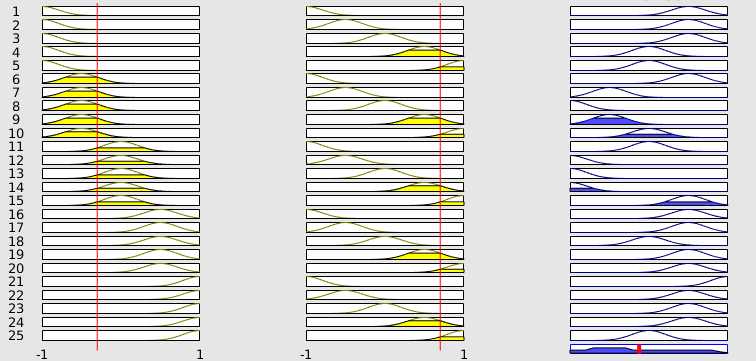
\includegraphics[width=0.5\linewidth]{figure/fuzzyeg}
\end{figure}

\paragraph{模糊控制仿真}
XXXX

\subsubsection{天棚阻尼}
XXXX



\subsection{实验模型设计}
\section{实验进展}
\subsection{MR阻尼器模型设计及理论计算}
\subsubsection{整体结构}
从工作模式来分,MR阻尼器主要有阀式、挤压流动式、剪切式、剪切阀式四种形式;从受力方式来分,可以分为单出杆和双出杆两种类型;从活塞相对于缸体的运动方式来看,可以分为直线型和旋转型。本组采用了剪切阀式、单出杆、直线型MR阻尼器。具体结构分析见图 \ref{mrdamper}。

\begin{figure}[H]
	\centering
	\bicaption{磁流变液阻尼器整体结构}{Overall structure of MR damper}
		{1:端盖; 2:缸壁; 3:线圈挖槽; 4:活塞杆; 5:阻尼通道; 6:磁芯}
		\label{mrdamper}
	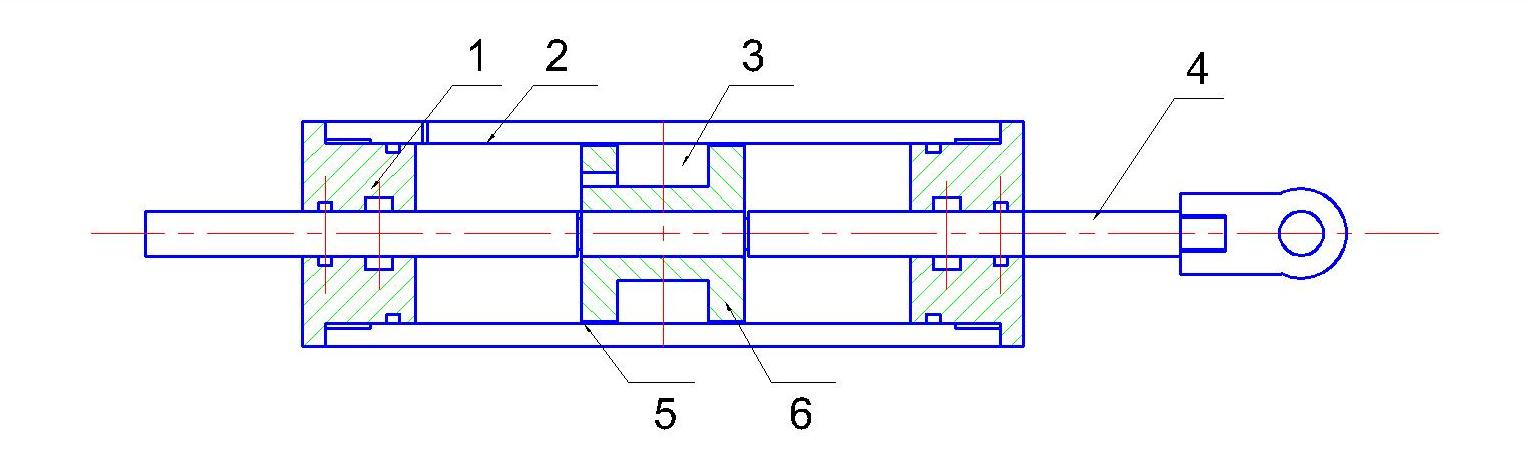
\includegraphics[width=6in]{figure/mrdamper}
\end{figure}

\subsubsection{材料选择}
\paragraph{磁流变液}
\qquad MRF(Magnetorheological fluid)是由大量的顺磁性颗粒悬浮于载体介质(如硅油),并添加一定量的抗沉降和抗凝结的添加剂混合而成。在无外加磁场的情况下,MRF可以简化为经典的牛顿黏性流体。在外加磁场作用下,MRF内部的顺磁性颗粒将发生极化,相互牵引形成链状结构,能够显著提高液体的表现黏度(apparent viscosity),大大增强垂直于磁场方向的液体剪切屈服强度(yield shear strength),且当外加磁场消失后,MRF能够重新转退回牛顿黏性流体。更为重要的是,MRF的剪切屈服强度能够由外加磁场强度的大小精确控制,是制作半主动控制装置的理想材料。

本组采用XXXXXXX,性质见表。

良好的MR阻尼器对MRF的性能有较高的要求:首先,由于MRF分散相粒径粗、比重大,长期静置后MRF中的顺磁性颗粒容易沉降,最终导致MRF丧失流动性功能。因此抗沉降和抗凝结的添加剂的质量和比例需要精确控制;其次,在实际的结构抗震环境中,MR阻尼器要承受的环境激励具有不可预知性,为了提供广泛的控制范围,MRF需要提供低零场黏度和高屈服力。最后,由于MRF在减振过程中受到来回剪切作用,要求MRF具备良好的散热性,且在长期的振动下不分层、不团聚、不发生明显的体积改变。

\paragraph{结构主体材料选取}

\qquad MR阻尼器的主要结构部件包括缸筒、活塞盘、活塞杆、端盖及励磁线圈等。

缸筒、活塞杆不仅是主要的受力构件,也参与阻尼器内部磁回路的组成。XX钢材不仅具备较高的机械强度,能够满足受力需求;同时具备较高的相对磁导率,饱和磁感应强度在1.5T以上,能够满足导磁性能的要求。

活塞盘作为磁回路重要的组成部分,要求材料具备良好的导磁性能,即较高的相对磁导率和饱和磁感应强度。电工纯铁是目前MR阻尼器活塞盘的主流材料。然而由于缺少该实验尺寸下的电工纯铁的标准件,单独加工成本较高。且实际地震波的频率大约在5Hz以内,磁感应强度方向变化慢,因此采用纯钢能够满足其导磁需求。因此采用纯钢作为活塞盘制作材料。

为了减少阻尼器在端盖部分发生漏磁现象,端盖采用不导磁的XX制作。

励磁线圈选用直径较大的漆包线,降低电阻,减少励磁线圈的发热量。

\subsubsection{参数设计}

设计过程中已知参数见表\ref{init}。
\begin{table}[H]
\bicaption{设计参数}{Design parameters}
\centering
\label{init}
\footnotesize
\begin{tabular}{|c|c|c|c|}
\hline 零场黏度$\eta$ & MRF屈服剪切应力$\tau_y$ & MRF饱和磁感应强度$B$ & 磁芯材料饱和磁感应强度$B_1$ \\
\hline $0.2Pa\cdot s$ & $68kPa$ & $0.6B$ & $1.5B$ \\
\hline 最大工作电流$I$ & 活塞最大速度$u$ & 空气磁导率$\mu_0$ & 阻尼通道饱和磁场强度$B_2$ \\
\hline $1.0A$ & $0.03m/s$ & $1.26\times10^{-6}H/m$ & $1.5T$ \\
\hline
\end{tabular}
\end{table}



根据磁路欧姆定律,剪切阀式MR阻尼器的磁路计算公式如式\eqref{NI}:
\begin{equation}
NI=\Phi\left(\frac{L^{'}}{\mu_1S_1}+\frac{2h}{\mu_0S_0}\right)=\Phi\left(R_{m1}+R_{m0}\right) \label{NI}
\end{equation}

式中,$N$为励磁线圈匝数;$I$为最大电流;$\Phi$为回路总磁通;$L^{'}$为磁路平均长度;$h$为阻尼通道宽度;$\mu_0$为空气磁导率;$\mu_1$为磁芯磁导率;$S_1$为磁路平均截面积;$S_0$为阻尼通道处平均截面面积;$R_{m1}$为磁路总磁阻;$R_{m0}$为阻尼通道总磁阻。由于$\mu_0$远小于$\mu_1$,因而$R_{m0}$远大于$R_{m1}$。

考虑磁路最优问题,避免活塞磁芯过早饱和,导致磁路浪费,本文假设间隙处的MRF在最大电流状态下能够达到磁饱和状态,即应满足式\eqref{Phi}。此外,假设磁芯处和阻尼通道处同时达到磁饱和状态,可建立磁路关系如式:
\begin{equation}
\Phi=BS_0\label{Phi}
\end{equation}
式中,$B$为MRF的饱和磁感应强度。

\begin{equation}
\Phi_1=\Phi_2\label{Phi1}
\end{equation}
\begin{equation}
\Phi_1=\pi r^2B_1\label{Phi2}
\end{equation}
\begin{equation}
\Phi_2=2\pi\left(r+h_1\right)L_1B\label{Phi3}
\end{equation}
式中,$\Phi_1$为磁芯处的饱和磁通;$\Phi_2$为阻尼通道处的饱和磁通;$B_1$为磁芯材料的饱和磁感应强度;$r$为磁芯半径;$h_1$为线圈槽挖深;$L_1$为活塞翼缘宽度。

由\eqref{Phi1}简化可得:
\begin{equation}
L_1=\frac{r^2B_1}{2\left(r+h_1\right)B}
\end{equation}

根据式\eqref{Phi},式\eqref{NI}可简化为式\eqref{N}。对于选定的MRF及最大工作电流,励磁线圈匝数$N$仅由阻尼通道宽度$h$确定。
\begin{equation}
N=\frac{2Bh}{\mu_0I}\label{N}
\end{equation}

本文采用剪切阀式直线型MR阻尼器,阻尼力计算公式可简化为:
\begin{equation}
F=F_{\eta}+F_{\tau}=\frac{12\eta LA{_p}{^2}}{\pi Dh^3}v+\frac{3L\tau_yA_p}{h}sgnv\label{F}
\end{equation}

式中:$F_{\eta}$为粘滞力;$F_{\tau}$为库仑阻尼力;$\eta$为MRF的零场黏度;$L$为活塞有效长度,即有效磁极宽度;$A_p$为活塞面积;$h$为活塞与缸体间的阻尼通道间隙;$D$为活塞外径;$\tau_y$为MRF的剪切屈服强度;$v$为活塞相对于缸体的运动速度。粘滞力与磁场强度无关,仅有MRF自身性质及活塞相对于缸体的运动速度有关,不可调控;库仑阻尼力在总阻尼力中比重较大,且可由磁场强度精确控制。

式\eqref{F}中各参数关系复杂,本文没有直接求解,而是编写程序,根据待定参数磁芯半径$r$和阻尼通道宽度$h$自动进行组合、迭代与测试,经过与加工厂商量,考虑模型的实际加工难度和成本,最终确定$r=11mm$、$h=1mm$及各项设计参数,见表\ref{element}。MR阻尼器活塞细部见图\ref{detail}。

\begin{table}[H]
\centering
\bicaption{设计尺寸}{Design size}
\label{element}
\footnotesize
\begin{tabular}{|c|c|c|c|}
\hline 活塞杆半径$r_0$ & 线圈槽挖宽$L_2$ & 活塞节段数$n$ & 磁芯半径$r$ \\
\hline $5mm$ & $20mm$ & $1$ & $11mm$ \\
\hline 阻尼通道宽度$h$ & 线圈槽挖深$h_1$ & 活塞翼缘宽度$L_1$ & 线圈匝数$N$ \\
\hline $1mm$ & $9mm$ & $8mm$ & $487$ \\
\hline

\end{tabular}
\end{table}

\begin{figure}[htb]
	\centering
	\bicaption{活塞细部图}{Detail structure of piston}
	\label{detail}
	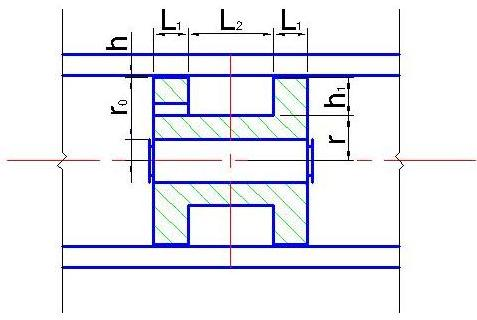
\includegraphics[width=4in]{figure/detail}
\end{figure}

根据表\ref{element}可以进一步计算各项参数如下:
活塞有效长度:
\begin{equation}
L=2nL_1=2\times1\times8mm=16mm
\end{equation}
活塞有效截面积:
\begin{equation}
\begin{split}
A_p&=\pi\left(h_1+r\right)^2-\pi r{_0}{^2}\\&=\pi\times\left(0.009+0.011\right)^2-\pi\times0.005^2=11.78cm^2
\end{split}
\end{equation}
阻尼通道平均周长:
\begin{equation}
\begin{split}
D^{'}&=2\left(r+h_1\right)+h\\&=2\times\left(11+9\right)+1=41mm
\end{split}
\end{equation}

根据式\eqref{F}可得:
\begin{equation}
\begin{split}
F_\eta&=\frac{12\eta LA{_p}{^2}}{\pi Dh^3}v\\&=\frac{12\times0.2\times0.016\times11.78^2\times10^{-4}}{\pi\times0.041\times0.001^3}\times0.03=17.40N
\\
F_{\tau}&=\frac{3L\tau_yA_p}{h}sgnv\\&=\frac{3\times0.016\times68000\times0.1178}{0.001}=3862.71N
\end{split}
\end{equation}

\subsubsection{阻尼器实物}
按照设计的材料、结构和参数,我们联系工厂配置了阻尼液,加工了阻尼器,得到试验用的磁流变阻尼器。

\begin{figure}[H]
	\centering
	\bicaption{磁流变液阻尼器实物}
		{MR damper}
	\label{shiwu}
	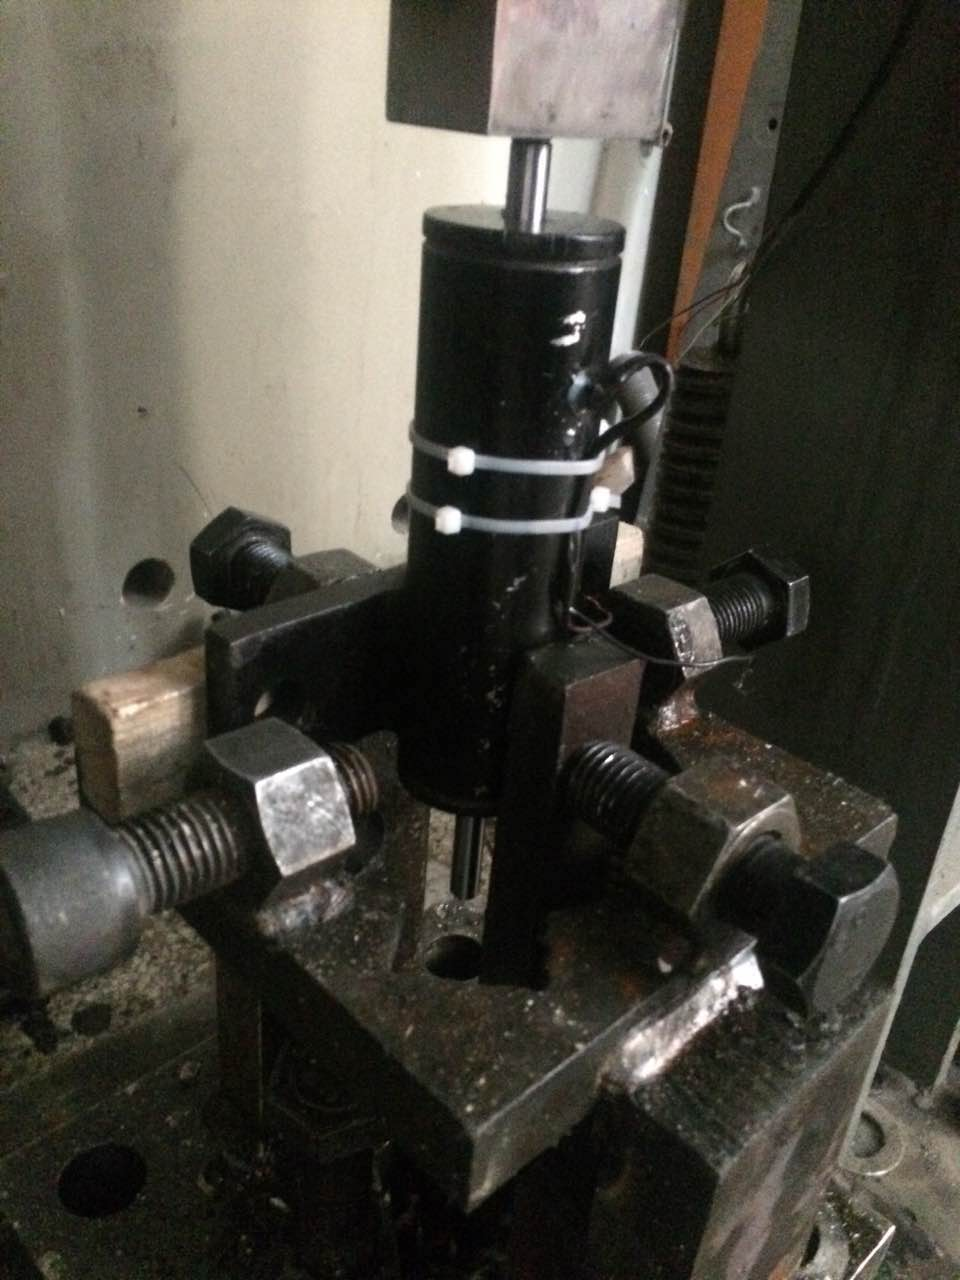
\includegraphics[width=.5\linewidth]{figure/shiwu}
\end{figure}

\subsection{MR阻尼器力学性质测试}

在磁流变阻尼器的实物制作完成后,由于制作材料的离散性、理论模型与实际情形的差异以及构件加工制作误差,我们需要对磁流变阻尼器的力学性能进行测试,以获得阻尼器真实的力学参数,为控制算法提供必要的输入参数,并未后期将要进行的模型试验的试验设计提供必要的参考依据。

测试试验主要包括两个方面的内容:

\begin{enumerate}
	\item 在不同的输入电流下对阻尼器进行循环加载试验,获得磁流变阻尼器的剪切屈服强度-输入电流相关曲线。根据相关学者的理论模型,磁流变阻尼器的剪切屈服强度与输入电流在一定范围内呈线性关系,并且由于粘滞流体的阻尼特性与阻尼器机械装置间的摩擦,线性曲线将具有一个正截距。
	
	\item 在构件制作时,由于材料限制,阻尼器中的导磁材料没有采用导磁性能良好的电工纯铁,而采用导磁性能稍逊的钢材。因此,当阻尼器的输入电流由高变低时,导磁材料中将不可避免地出现剩磁现象,导致阻尼器的剪切屈服强度无法迅速回到期望水平,而是必然存在延迟。为了保证控制算法的输出的准确性,有必要考虑这种延迟效应,并将其定量化。
\end{enumerate}

循环加载试验的加载幅值为20mm,峰值加载速度为0.6m/s,测试试验定于3月12日进行。



\begin{figure}[H]
	\centering
	\bicaption{磁流变液阻尼器滞回曲线测试}
		{Experiment on the hysteresis curve of MR damper}
	\label{shiyan}
	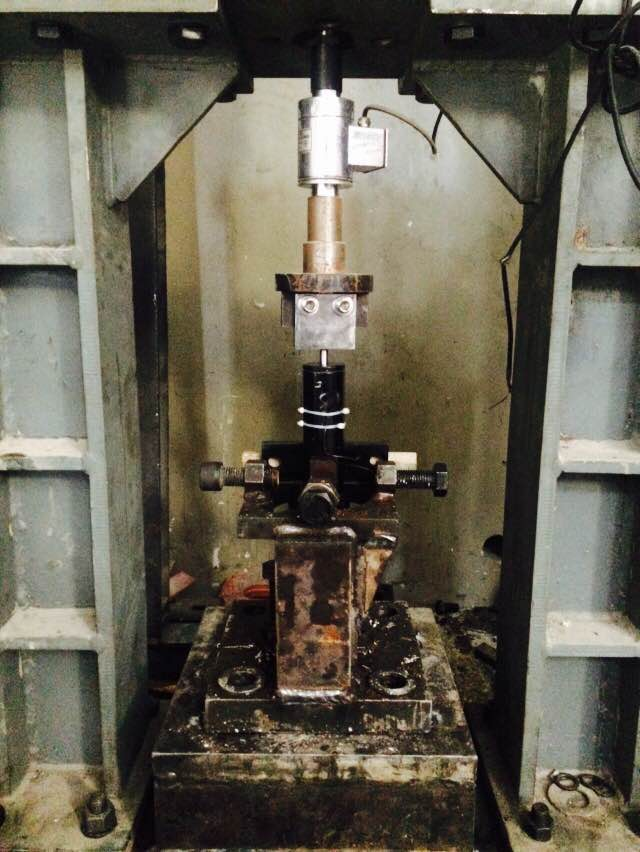
\includegraphics[width=.5\linewidth]{figure/shiyan}
\end{figure}








\subsection{半主动控制系统搭建}

\begin{figure}[H]
	\centering
	\bicaption{中文}
		{English}
	\label{arduino}
	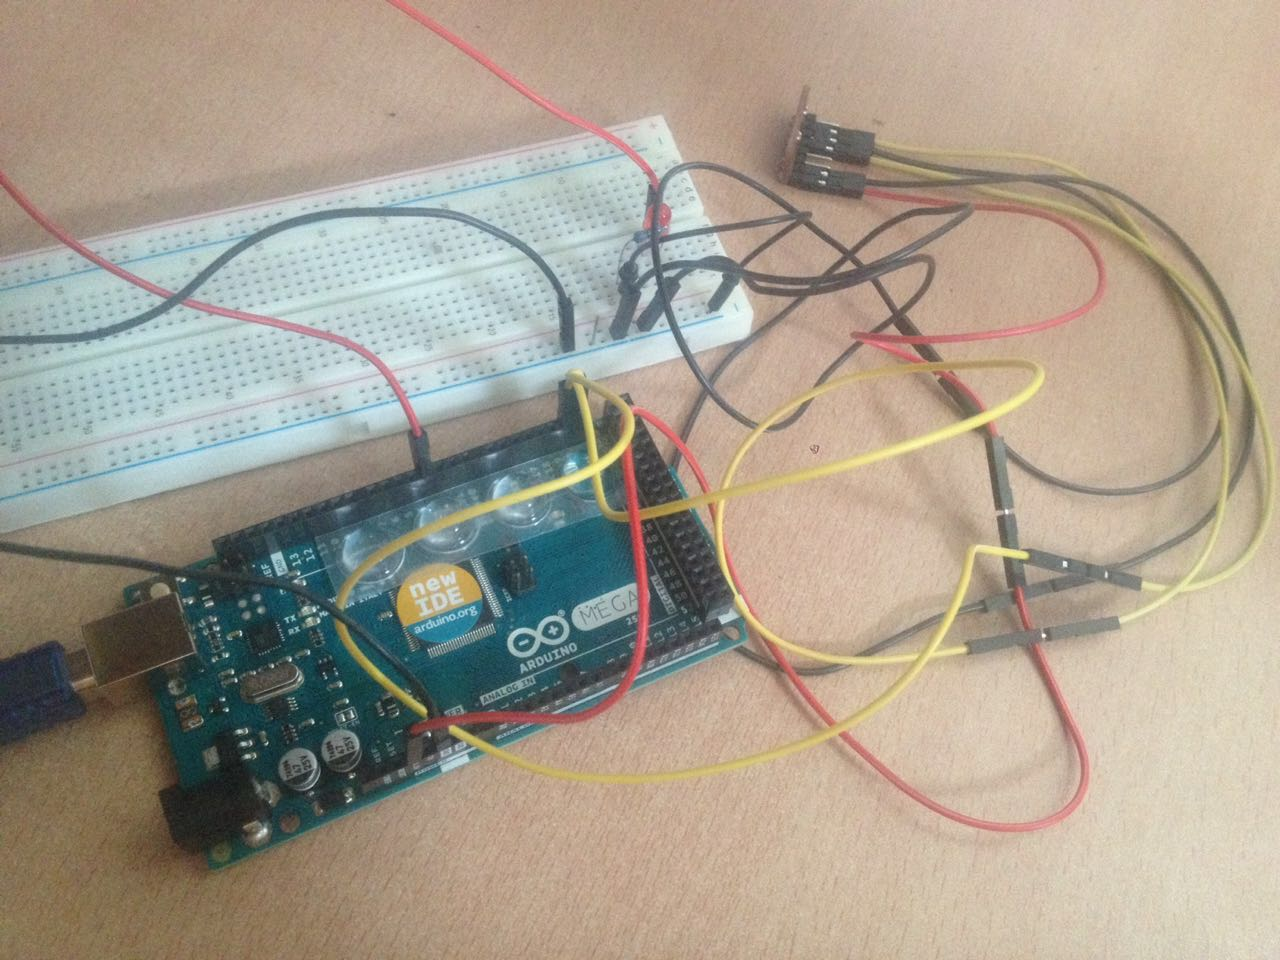
\includegraphics[width=.5\linewidth]{figure/arduino}
\end{figure}




\subsection{直线型发电机设计}
基于法拉第电磁感应定律,闭合回路中的一部分导体,在磁场中运动时,在导体两端会产生感应电动势,并且感应电动势与回路中磁通量的变化率成正比\cite{elliott1993},见式\eqref{magE}。

\begin{equation}
\label{magE}
E=\frac{d\Phi}{dt}
\end{equation}

结合双出型MR阻尼器的机械构造,设计直线型发电机如图\ref{powerstation}所示。该装置由磁漏罩、定子系统与动子系统组成。定子系统包括定子与线圈,线圈绕在定子的凹槽内。动子系统包括永磁体、衔铁与动子连接杆,动子连接杆一头与MR阻尼器双出杆一头相连,永磁体与衔铁相邻布置,为提高发电效率,相邻永磁体极化方向相反,如图\ref{simu}所示磁感线近似成矩形。结构在振动时,动子通过动子连接杆与结构连接,与定子产生相对运动,改变线圈内磁通量,从而产生电能。磁漏罩位于装置最外侧,由不导磁材料制成,减少磁漏。

\begin{figure}[H]
\centering
\bicaption{直线型发电机模型}{Linear generator model}
\label{powerstation}
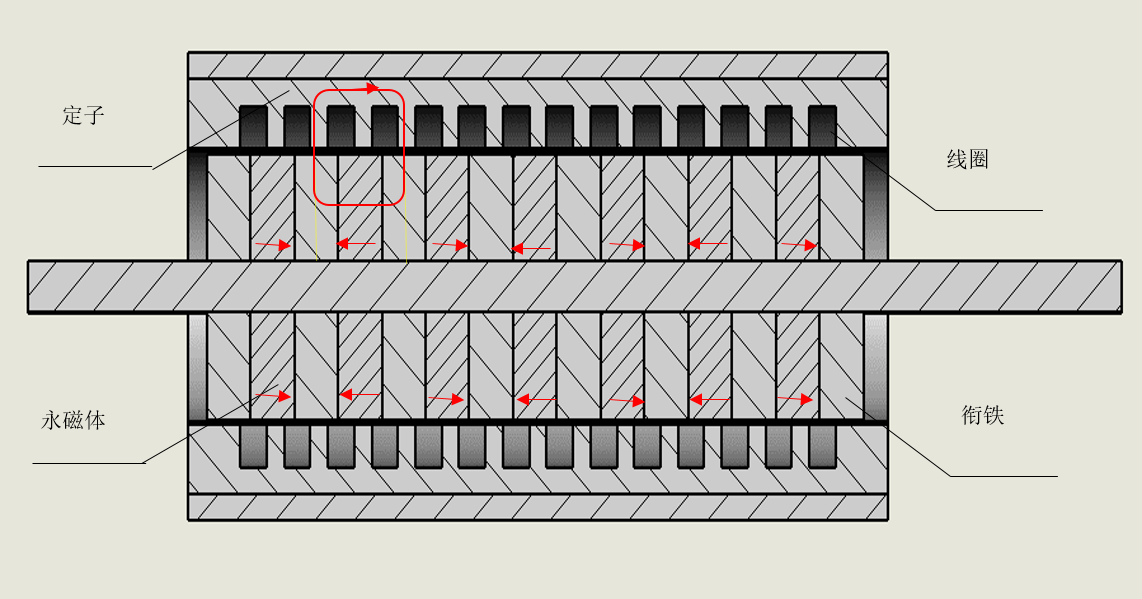
\includegraphics[width=4in]{figure/straight}
\end{figure}

为了能够在低频振动的条件下,收集足够多的电能,在该设计中采取了一系列措施来增大线圈内的磁场强度,防止磁场泄露,提高发电效率:

\begin{enumerate}[leftmargin=*,labelindent=16pt,label=\bfseries \arabic*.]
	\item 采用磁场最强的汝铁硼稀土永磁体材料NdFeB-N50作为永磁体。NdFeB-N50的最大磁能积可达$415kJ/m^3$,利用其产生高强磁场,大大提高发电效率;
	\item 在永磁体排布时,使相邻永磁体极化方向相反,两片永磁体之间用软钢衔铁连接,利用两块永磁体相反的磁动力,迫使磁感线沿装置径向扩散,穿过线圈形成磁回路,提高磁场利用率;
	\item 将线圈分隔成十四个小线圈,每个线圈独立发电,整流后输出电能,充分利用永磁体产生的磁场,提高发电效率;
	\item 设置磁漏罩套于定子外部,磁漏罩由不导磁的铝材料组成,阻止磁感线向外部泄露,迫使磁感线穿越线圈形成闭合回路,用于产生感应电动势。
\end{enumerate}

为进一步验证模型的可行性,在Ansoft Maxwell软件中建立装置模型进行仿真模拟分析。线圈、气隙与塑料筒相对磁导率与真空接近,设置为1;定子及衔铁选用软钢材料,在Maxwell中设置为材料Steel\_1008;磁漏罩与动子连接杆选用不导磁的铝材料,在Maxwell中设置材料为Aluminum;对于永磁体材料,通过自身$B-H$曲线进行定义。

图\ref{simu}所示的是永磁体产生的磁感线在设计装置中的分布图,由模拟结果可见,磁感线的分布与我们设想的基本一致,绝大部分磁感线都能够穿过“气隙—定子T型齿—定子”形成磁感线闭合回路,磁感线形状近似为矩形。当动子与定子产生相对运动时,线圈切割磁力线回路,产生感应电动势。理论仿真所得气隙内磁感应强度平均大小约为$1.157T$,可以达到理论要求。

\begin{figure}[htb]
	\centering
	\bicaption{磁感线分布图}{Distribution map of magnetic induction line}
	\label{simu}
	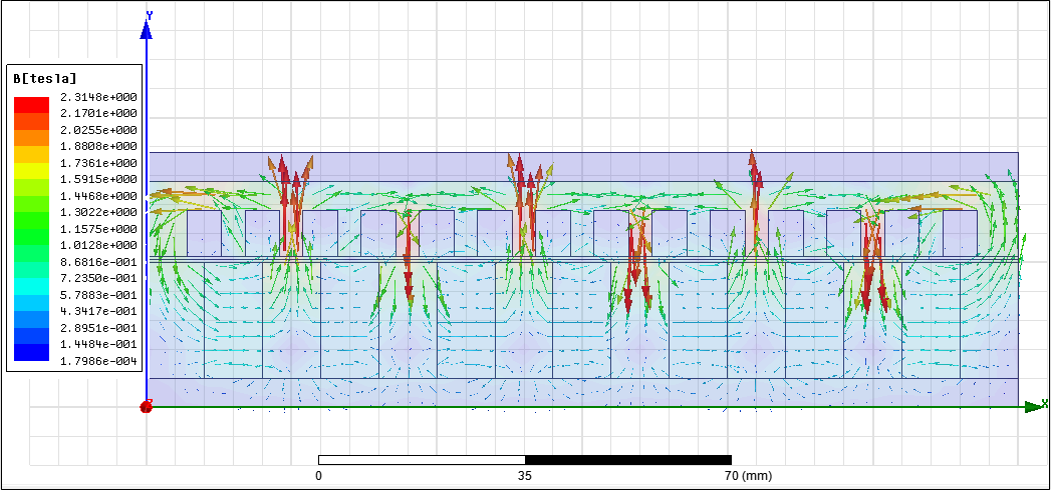
\includegraphics[width=5in]{figure/simu}
\end{figure}

通过理论仿真,我们初步验证了该发电装置的可行性,现阶段该模型已绘制详细图纸交由厂家制作,由于生产过程中存在较多不确定因素,该发电装置的理论发电量计算与试验分析将在后续报告中进行详细阐述。
\section{下一步工作}

接下来的工作将围绕着试验平台的搭建以及模型试验展开。目前,模型试验控制电路的设计搭建已基本完成,仅需要对发电装置的稳压模块进行更进一步的优化。

由于我们制作的磁流变阻尼器的出力远小于实际建筑结构的需求,因此现有的结构振动装置不能用于模型试验,同时,其出力又大于小型振动台的工作范围,并且小型振动台的低频输出并不稳定,难以用于进行模型试验,因此,需要特别搭建试验平台,目前,试验平台的振动装置仍在制作。


%---------------------------------
%参考文献

\bibliographystyle{plain}
\bibliography{bibtex/report}

%---------------------------------
\end{document}
